\documentclass{article} 
\usepackage{geometry} 
\usepackage{hyperref} 
\usepackage{graphicx} % For including graphs
\geometry{a4paper, margin=1in}

\begin{document}
\begin{titlepage}
\centering
\vspace{1em}
\fontsize{14}{16}\selectfont % Set font size to 14
\textbf{CS371L - Artificial Intelligence}

\vspace{2.5em}

\fontsize{24}{26}\selectfont % Set font size to 24
\textbf{Real Time Sign Language Translation}
\vspace{1.5em}



\includegraphics[width=0.3\linewidth]{UET_logo.png} \\
\fontsize{10}{12}\selectfont % Set font size to 10
\caption{Session: 2022 – 2026}

\vspace{4em}

\fontsize{16}{18}\selectfont % Set font size to 16
\textbf{Submitted by:} \\

\vspace{0.5em}

\fontsize{15}{18}\selectfont % Set font size to 15
Muhammad Tayyab      \hspace{1.5em}           2022-CS-133

\vspace{3em}

\fontsize{16}{18}\selectfont % Set font size to 16
\textbf{Submitted To:} \\

\vspace{0.5em}

\fontsize{15}{18}\selectfont % Set font size to 15
Mr. Numan Shafee

\vspace{4em}

\fontsize{18}{20}\selectfont % Set font size to 15.5
Department of Computer Science \\
\fontsize{22}{25}\selectfont % Set font size to 15.5
\textbf{University of Engineering and Technology Lahore Pakistan}
\end{titlepage}


\section*{1. Objective} 
The objective of this project is to build an AI-based system that can translate sign language into spoken language in real time using video input. This system aims to facilitate communication between deaf and hearing individuals by recognizing hand gestures and mapping them to words or phrases using machine learning models.

\section*{2. Background and Motivation} 
\begin{itemize}
    \item Motivation: Communication barriers for individuals who rely on sign language create challenges in many settings, including education, healthcare, and everyday interactions.
    \item Proposed Solution: Leveraging recent advances in deep learning and computer vision, we aim to enable real-time translation of sign language into spoken language.
    \item Technological Foundation:
        \begin{itemize}
            \item CNNs for gesture recognition to detect spatial patterns.
            \item RNNs (LSTM/GRU) for modeling temporal dependencies in the sequence of gestures.
        \end{itemize}
    \item Social Impact: This project aims to enhance accessibility and inclusivity, providing a solution for communication between deaf and hearing individuals.
\end{itemize}

\section*{3. Proposed Methodology} 
We will approach the project in several structured steps to ensure a smooth development process.

\subsection*{Data Collection} 
\begin{itemize}
    \item Source: Publicly available sign language datasets (e.g., American Sign Language dataset).
    \item Custom Dataset: If needed, we will generate our own dataset using video recordings.
    \item Annotation: Each gesture will be labeled with its corresponding sign or phrase for model training.
    \item Data Augmentation: Techniques like image rotation, flipping, and scaling will be applied to increase dataset variability.
\end{itemize}

\subsection*{Algorithms/Models} 
\begin{itemize}
    \item CNN (Convolutional Neural Networks):
        \begin{itemize}
            \item CNNs will be used for feature extraction from individual video frames.
            \item Pre-trained CNNs (e.g., InceptionV3, ResNet) can be fine-tuned for gesture classification.
        \end{itemize}
    \item RNN (Recurrent Neural Networks):
        \begin{itemize}
            \item RNNs (LSTM or GRU) will capture the sequential nature of gestures, enabling accurate interpretation of sign language phrases.
            \item The RNN will handle temporal dependencies between gestures to form complete sentences.
        \end{itemize}
\end{itemize}

\subsection*{System Workflow}
\begin{itemize}
    \item Video Input: Capture real-time video using a webcam.
    \item Hand Gesture Detection: Detect hand gestures using OpenCV and MediaPipe.
    \item Gesture Classification: Use CNN to classify individual frames.
    \item Temporal Modeling: Use RNN to analyze the sequence of gestures for full phrase translation.
    \item Speech Output: Convert the recognized sign language into spoken words using a text-to-speech system.
\end{itemize}

\subsection*{Flow Diagram}
Below is a placeholder for a flow diagram that illustrates the system architecture:
\begin{figure}[h]
    \centering
    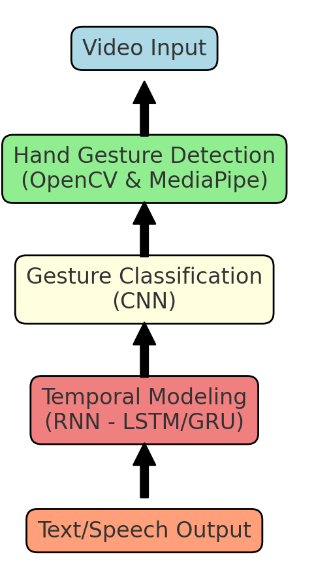
\includegraphics[width=0.5\textwidth]{Screenshot 2024-10-13 180653.png}
    \caption{System Architecture Flow Diagram}
    \label{fig:flowchart}
\end{figure}

\subsection*{Tools and Technologies} 
\begin{itemize}
    \item Python: The primary programming language for implementation.
    \item Libraries:
        \begin{itemize}
            \item \texttt{TensorFlow} and \texttt{Keras} for model development.
            \item \texttt{OpenCV} for real-time video processing.
            \item \texttt{MediaPipe} for hand tracking and gesture detection.
        \end{itemize}
    \item Hardware: A standard webcam for video input.
\end{itemize}

\subsection*{Evaluation Metrics} 
\begin{itemize}
    \item Accuracy: Overall performance in correctly translating gestures into words.
    \item Precision and Recall: Measures of how well the model identifies correct gestures and avoids false positives.
    \item F1-Score: The harmonic mean of precision and recall, providing a balance between both.
    \item Latency: Time taken to translate gestures in real time.
    \item Word Error Rate (WER): Measures how often the recognized words deviate from the correct translation.
\end{itemize}

\section*{4. Expected Outcomes} 
\begin{itemize}
    \item Goal: A working prototype capable of real-time sign language translation with high accuracy.
    \item Challenges:
        \begin{itemize}
            \item Variability in signing speed and gestures.
            \item Regional variations in sign languages.
        \end{itemize}
    \item Potential Applications:
        \begin{itemize}
            \item Healthcare communication between doctors and deaf patients.
            \item Educational tools for sign language learners.
            \item Public service accessibility improvements.
        \end{itemize}
\end{itemize}

\section*{5. References} 
\begin{itemize}
    \item Intelligent Predictive Model for Hepatitis C, 2023 \cite{ref1}.
    \item Cleft Prediction Before Birth Using Deep Neural Networks, 2020 \cite{ref2}.
    \item Deep Learning for Sign Language Recognition Using CNN and RNN, 2022 \cite{ref3}.
    \item MediaPipe Documentation on Hand Detection, 2021 \cite{ref4}.
    \item Real-Time Gesture Recognition with OpenCV, 2020 \cite{ref5}.
\end{itemize}

\section*{6. Conclusion} 
By the end of this project, we aim to demonstrate a fully functional prototype capable of real-time sign language translation. This solution will contribute to improving communication for individuals who use sign language, fostering greater inclusion in society.

\end{document}